\documentclass[12pt]{article}

\usepackage{geometry}
 \geometry{
 a4paper,
 left=25mm,
 right=20mm,
 top=20mm,
 }
 
\usepackage{hyperref}
\usepackage{exercise}
\usepackage{enumerate}
\usepackage{graphicx}
\usepackage{subfig}
\usepackage{listings}
\usepackage{tikz}

\usepackage{amsmath}
\usepackage{amsfonts}

\usetikzlibrary[topaths]

\renewcommand{\baselinestretch}{1.2}

%\usepackage[active,tightpage]{preview}

%\PreviewEnvironment{tikzpicture}
%\setlength\PreviewBorder{5pt}

\newcommand\MyFive[2]{%
  \foreach \x in {1,...,5}{
    \pgfmathparse{(\x-1)*72+floor(\x/6)*36 + 90 - 90*#2}
    \node[draw,circle,inner sep=5pt,text width=1cm, align=center] (#1-\x) at (\pgfmathresult:2.5cm){ \ifthenelse{1 = \x}{Master Node}{Node $\x$}};
  }
  \foreach \x [count=\xi from 1] in {1,...,5}{
    \foreach \y in {\x,...,5}{
    \path (#1-\xi) edge[-] (#1-\y);
  }
}
}


\lstset{language=erlang, firstline=37, lastline=45, title={Listing 1: Data structures for cellular automaton}}

\begin{document}

\title{
Distributed Systems \\
\textbf{Building a Middleware for Distributed System in Erlang}\\
Project report
}

\author{Ievgeniia Oshurko}
\date{April 16, 2016}
\maketitle


\section{Introduction}

In this project a middleware for distributed system was implemented. The main function of the middleware is to manage cluster consisting of connected remote nodes. This cluster can be used for handling big load of small tasks. 


\textbf{Topology}. The remote nodes are connected into clique topology forming a fully connected network so that all nodes have direct links to other nodes. \emph{Why clique topology has been chosen?} Clique topology has an overhead in the number of  connection links, but at the same time it is highly fault tolerant. In case of crash of any node in the network, its topology does not change, and all nodes stay connected. Consider the performance requirements for our distributed system: we want a huge number of incoming small jobs to be distributed into our system efficiently. As master node has direct link to each node, it takes exactly one hop for master to send a message to any node. In case of clique topology we do not need to broadcast a message, as well. \emph{Why don't consider a star topology?} In case of star topology if the master node dies, it becomes impossible to recover the system functioning. In case of master node crash in clique topology the network is still functioning, and upon detection of the crash of master node other nodes can, for example, elect new master among them and continue work, reporting to the system monitor that new master node has been chosen (so the entry point changed).

On the figure below example of implemented clique topology is illustrated. 

	\begin{center}
		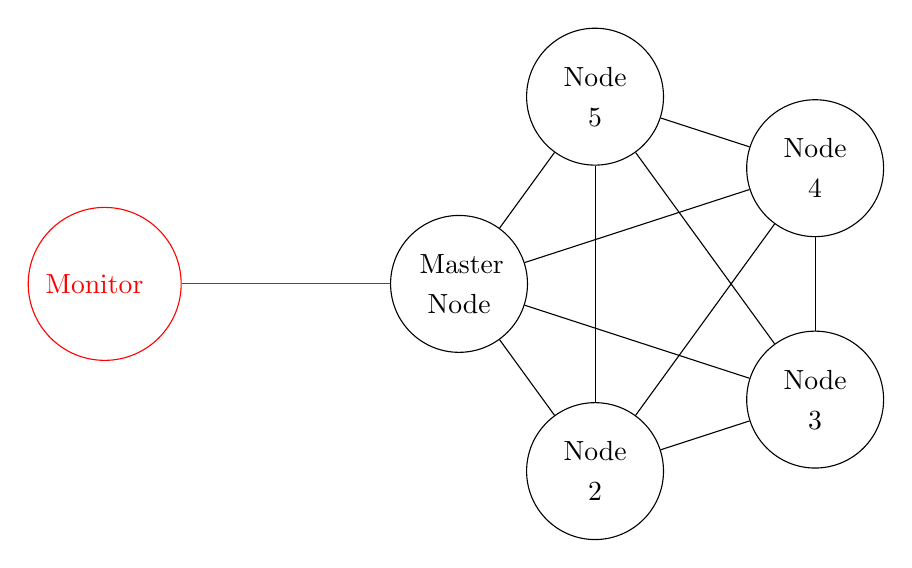
\begin{tikzpicture}
			\node[draw,circle,inner sep=5pt,text width=1.5cm,color=red](Monitor1){ Monitor };
			\begin{scope}[xshift=7cm]
			 \MyFive{A}{-1}
			\end{scope}
			\draw[red] (Monitor1) -- (A-1);
		\end{tikzpicture}
	\end{center}

To scale our system the following could be done: we can create multiple subclusters as previously described, and connect their master nodes with links, so that they can communicate and, for example, elect the least busy subcluster to exacute the tasks arriving from the side of monitor. 

	\begin{center}
		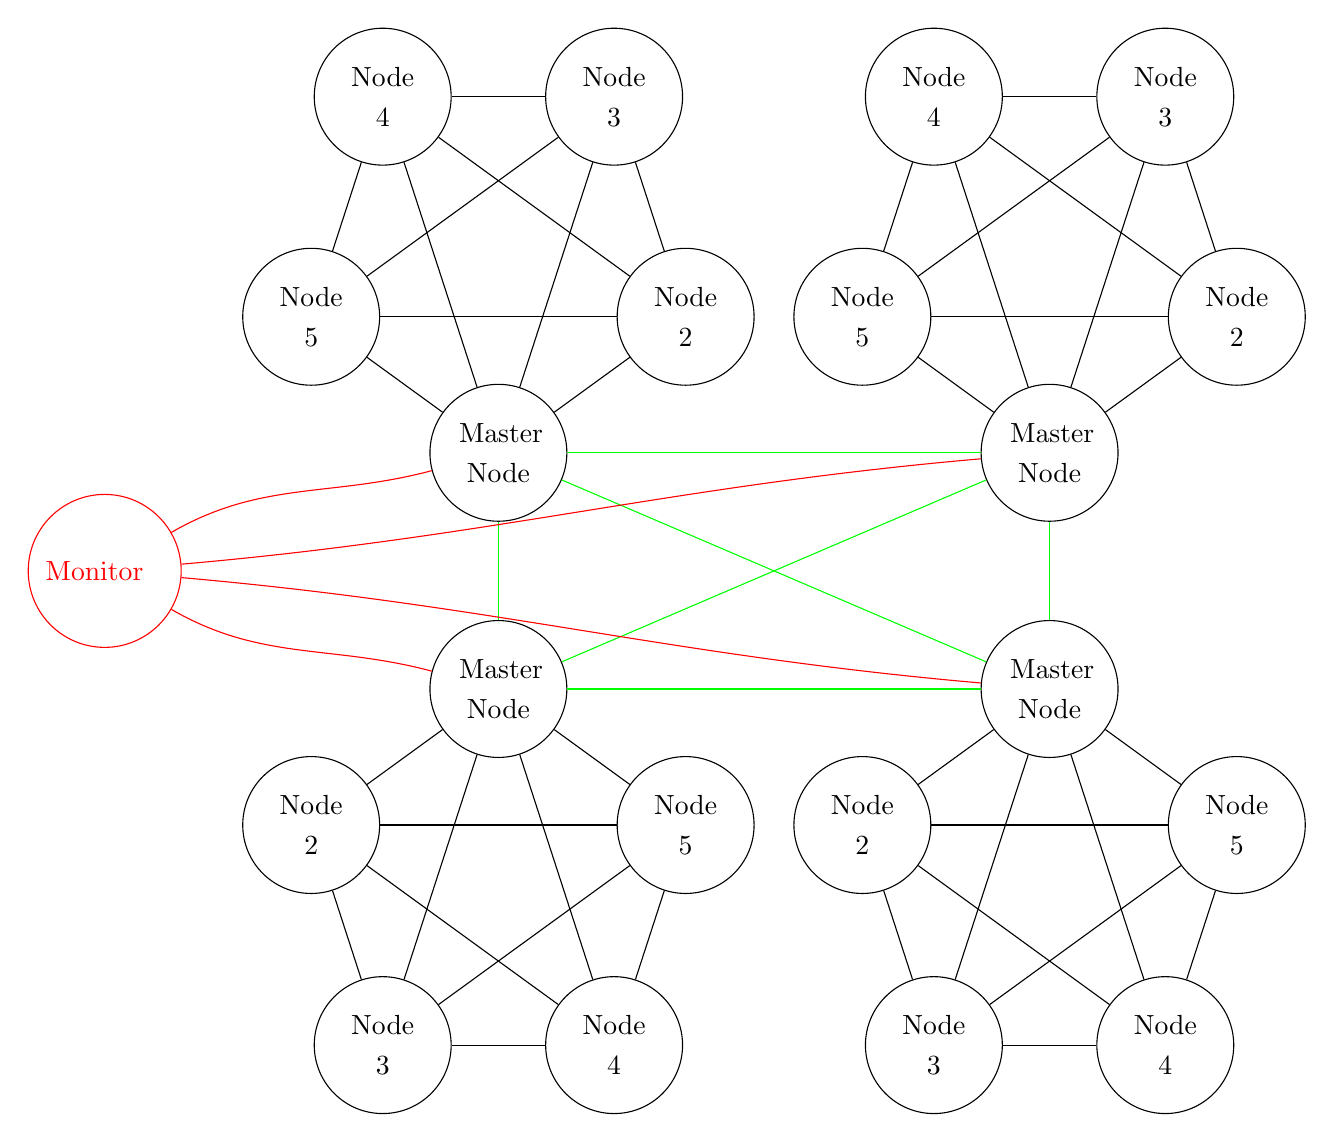
\begin{tikzpicture}
			\MyFive{B}{2}
			\begin{scope}[xshift=7cm]
			 \MyFive{C}{2}
			\end{scope}
			\begin{scope}[xshift=-5cm, yshift=-4cm]
			\node[draw,circle,inner sep=5pt,text width=1.5cm,color=red](Monitor2){ Monitor };
			\end{scope}
			\begin{scope}[yshift=-8cm]
			 \MyFive{D}{0}
			\end{scope}
			\begin{scope}[xshift=7cm, yshift=-8cm]
			 \MyFive{E}{0}
			\end{scope}
			\draw[green] (B-1) -- (C-1);
			\draw[green] (D-1) -- (E-1);
			\draw[green] (B-1) -- (D-1);
			\draw[green] (C-1) -- (E-1);
			\draw[green] (B-1) -- (E-1);
			\draw[green] (D-1) -- (C-1);
			\draw[red] (Monitor2) to[out=30, in=195] (B-1);
			\draw[red] (Monitor2) to[out=5, in=-175] (C-1);
			\draw[red] (Monitor2) to[out=-30, in=165] (D-1);
			\draw[red] (Monitor2) to[out=-5, in=175] (E-1);
		\end{tikzpicture}
	
	\end{center}


\textbf{Middleware Structure}. Implemented module consists of two submodules: \texttt{agents} and \texttt{monitor}. Submodule \texttt{monitor} implements the client interface for managing the system: start/stop cluster, add/remove new node, send job to execute, get cluster statistics. Monitor has an access to cluster through master node address. You can access to the cluster from multiple monitors. Each monitor process needs to be registered, so that master agent knows were to send the response (it needs process name and node address). Submodule \texttt{agents} contains the deamons that should be compiled and launched on nodes in order to start up implemented system. 

Implementation details and examples of usage are presented in the sections below.

\section{Agent deployment}

For each node in a cluster two processes spawned and registered under the names \emph{agent} and \emph{computing unit}:
\begin{itemize}
	\item \emph{agent} process runs daemon function \texttt{local\_agent\_loop} (or \texttt{master\_agent\_loop} in case of master node), which performs exchange of messages between the nodes, mostly communicating with master nodes and its computing unit. The agent also stores the queue of jobs to be executed on the node.
	\item \emph{computing unit} process runs daemon function \texttt{computation\_loop}, which communicates with its agent, performs job execution and sends back the results to agent.
\end{itemize}

Master node has special \emph{agent} that communicates not only with other nodes in cluster, but also with monitor, and receives from it special commands.

\subsection{Start/stop a cluster}

Monitor function \texttt{start\_cluster} takes as an input address of remote node and creates master node agent on it. At this point the cluster with single node (master) is started. It is also possible to call this function with two arguments: master node address and list of slave nodes addresses. In this case cluster topology with master and slave agents is created and is ready to receive jobs.

Cluster can be stopped using \texttt{stop\_cluster} monitor function, which sends stop message to the master node, then master node sends this message to all other nodes in cluster. When the node receives message to stop, it terminates computing unit process, unregisters it and unregisters its agent process. 

\subsection{Adding the nodes}

Function \texttt{add\_node} takes as an input master node address (cluster entry point) and the address of new node to be added. This function sends a special message to master node containing an address of new node. Master agent upon the receival of this message pings the node by the address, spawns agent daemon on this node (when slave agent daemon starts, it spawns computing unit process on the node). After this master agent informs all other nodes in topology about new node and adds this node to the list of agents alive.

\subsection{Removing the nodes}

Two functions of node removal are implemented: \texttt{pop\_node} and \texttt{remove\_node}. Function \texttt{pop\_node} allows us to delete the last added node, and \texttt{remove\_node} to remove specified node. In both cases master agent notifies all the nodes about the node removal, redistributes its job queue between other nodes (mechanism of jobs distribution will be discussed later) and after that removes it from the list of nodes alive, stops computing unit process and unregisters agent and computing unit.

\section{Remote job execution}

Our monitor should be able to send the jobs for execution from client to the cluster. It can be done using monitor function \texttt{execute\_job}, which sends the job to master node.

\subsection{Distribution of jobs}

When the master node receives the job for execution it needs to elect the node to perform the job (including itself). So, master sends a request to each node agent asking about the number of jobs in the node's queue. After this, master agent waits to receive all the queue lengths from the nodes, finds a node with the minumum queue length, and sends the job to it. The distribution of tasks is implemented is such a way that if master node and some other node have the same number of jobs in the queue, and it is minimal, the priority of job execution goes to other node, as we assume that master node is always more busy than other nodes with communication to other nodes and outer world.

\subsection{Job managing}

When particular node receives job to execute it is added to agent's job queue. The execution of jobs from the queue is implemented the following way: if the queue is empty and new job was received, it is automatically sended to node's computing unit execution. When the execution is finished, computing unit sends the message 'finished' with the result of computations to its agent, agent deletes this job from its queue and send the new job to computing unit. So, as you can observe, job is not deleted from the queue upon sending to computing unit, it stays there untill result is received -- it guaratees that when the node is removed, no jobs are lost, but all of them are rebistributed between other nodes.

\section{Agent monitoring}

Agent monitoring can be performed using the following functions: \texttt{get\_nodes} and \texttt{show\_nodes\_\\history}. Function \texttt{get\_nodes} returns the list of nodes currently alive in the cluser.

Function \texttt{show\_nodes\_history} gives us more information about cluster status. Master agent is implemented is such a way that it preserves its historical status, i. e. we can see which nodes are alive now, which were removed, and which nodes died. Master agent stores a dictionary with nodes and its' statuses, and updates this dictionary upon every change in the cluster: removal of node, death of node, etc.

It is implemented for security reasons: if some node was accidentally removed during the work with monitor or some node died, you still have the address to this node stored and you can add it to the cluster again.

Example of output:

\texttt{Cluster status: }

\texttt{================}

\texttt{Master Node: 'node1\_1@host'}

\texttt{--- 'node4\_1@host' : alive}

\texttt{--- 'node3\_1@host' : removed}

\texttt{--- 'node2\_1@host' : dead}



\subsection{Nodes status}

Master and slave agents are implemented in such a way that they check connection with other nodes at the beggining of each daemon loop iteration. Having this, unexpected death of node may cause troubles only in case it happens during the execution of some part of the loop iteration that is sending or receiving something. For this case agent daemons check the status of nodes not only at the beggining of each loop, but also every time they send/recive something.

\subsection{Death of master node}

Death of master node is still rather dramatical event as master node is the only entry point for our monitor. After the death of monitor the system will still be functioning, executing the tasks from its queue, and sending them to master node (so the results will never be received by client). What can be also implemented is that if master node is not reachable, the executed tasks are never deleted from the queue, and loop untill some master node will be connected or elected and receive the results of job execution.

Another thing that may be implemented as a solution of master death problem is the following. Assuming we have the list of nodes in the cluster that are still alive, we can start a master agent on a new node, and reconnect the nodes to it, without aborting the deamons running on them (aka without loosing job queue and other information they possess).

\section{Examples and applications}


Fault tolerant

Couple of examples where implemented. Script that deploy the middleware on the nodes, so they are ready to recieve the job.

Application: there is no distribution on task level - so each task is executed by a single node. The system is suitable for application where the number of incoming tasks, as it distributes them equally between the nodes. Smth like Web-server with numberous request from clients.


\end{document}
